\documentclass{article}
\usepackage{amsfonts}
\usepackage{amssymb}
\usepackage{amsmath}
\usepackage{amsthm}
\usepackage{float}
\usepackage{graphicx}
\usepackage{enumerate}
\usepackage[margin=1in]{geometry}
\usepackage{tikz}
\usepackage[T2A]{fontenc}   % Cyrillic font encoding
\usepackage[utf8]{inputenc} % Support for UTF-8 input
\usepackage[english,ukrainian]{babel}
\usepackage{listings}
\usepackage{xcolor}
\usepackage{subfigure}
\usepackage{hyperref}

\lstdefinelanguage{TypeScript}{
  keywords={class, export, boolean, throw, implements, import, this, switch, var, if, in, while, for, else, any, number, string, as, extends, enum, const, constructor, private, public, get, set, new, try, catch},
  sensitive=true,
  comment=[l]{//},
  morecomment=[s]{/*}{*/},
  morestring=[b]',
  morestring=[b]",
  keywordstyle=\color{blue}\bfseries,
  identifierstyle=\color{black},
  commentstyle=\color{green}\ttfamily,
  stringstyle=\color{orange}\ttfamily,
}

\lstset{
    language=TypeScript,
    basicstyle=\ttfamily\small,
    numbers=left,
    numberstyle=\tiny,
    stepnumber=1,
    numbersep=10pt,
    backgroundcolor=\color{gray!10},
    tabsize=2,
    showspaces=false,
    showstringspaces=false
}

\begin{document}

\begin{figure}[h!]
\centering
\includegraphics[width=8cm]{img/image1.jpeg}
% \caption{Example Image}
\label{fig:example}
\end{figure}
\begin{center}
Міністерство освіти і науки України Національний технічний університет України
\end{center}
\begin{center}
    «Київський політехнічний інститут»
\end{center}
\vspace{4cm}
\begin{center}
\Large \textbf{Лабораторна робота №3}
\end{center}
\begin{center}
    \textbf{з дисципліни «Алгоритми та методи обчислень»}
\end{center}
\vspace{4cm}

\hspace*{8cm} Виконав студент групи: КВ-22 \par
\hspace*{8cm} ПІБ: Крутогуз Максим Ігорович \par
\hspace*{8cm} Варіант 12 \par
\hspace*{8cm} Перевірив: 

\vspace{7cm}
\begin{center}
    \textbf{Київ 2024}
\end{center}


\begin{figure}
\centering
\includegraphics[width=0.7\textwidth]{AMO/img/lab3variantMethod.png}
\caption{Метод розв'Язання СЛАР за варіантом}
\label{fig:var1}
\end{figure}

\begin{figure}
\centering
\includegraphics[width=0.7\textwidth]{AMO/img/lab3varientMatrix.png}
\caption{Матриця за варіантом}
\label{fig:var2}
\end{figure}

\section{Реалізація алгоритм виключення за Гауссом}

\begin{figure}
\centering
\subfigure[Вхідна матриця]{
  \includegraphics[width=0.45\textwidth]{AMO/img/lab3lss1.png}
}
\hspace*{\fill} % Add space between subfigures
\subfigure[Результат]{
  \includegraphics[width=0.45\textwidth]{AMO/img/lab3lsa1.png}
}
\caption{Перевірка результатів на онлайн калькуляторі}
\label{fig:ls1}
\end{figure}

Для перевірки коректності алгоритму було перевірка коректності результату. Правильний результат можна побачити на рисунку \ref{fig:ls1}

Результат виконання програми можемо побачити на рисунку \ref{fig:gauss}

Блок-схема алгоритму можна побачити на рисунку \ref{fig:gaussfc}

\begin{figure}
\centering
\includegraphics{AMO/img/lab3gaussRes.png}
\caption{Результат алгоритму Гауса}
\label{fig:gauss}
\end{figure}

\begin{figure}
\centering
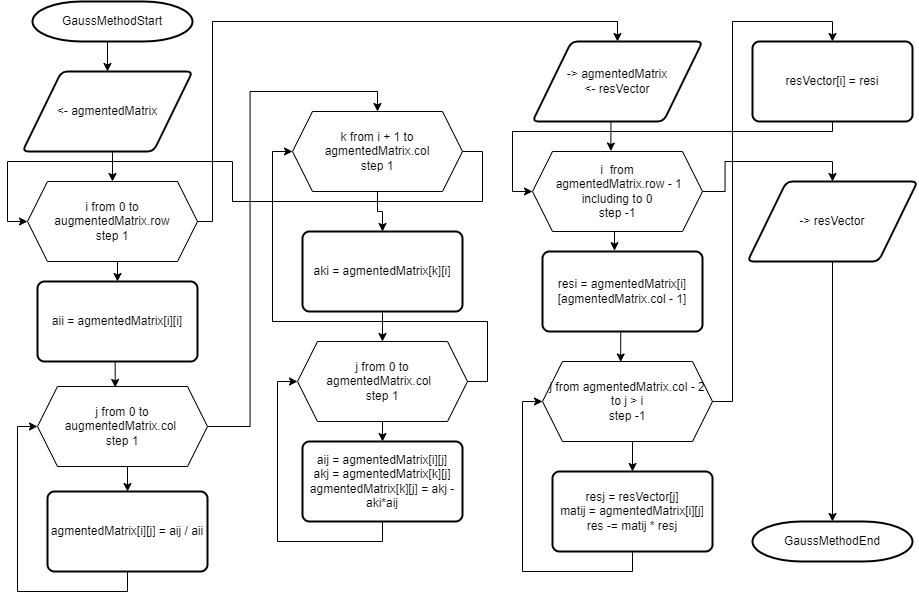
\includegraphics[width=0.9\textwidth]{AMO/img/Gauss.png}
\caption{Блок-схема алгоритму Гауса}
\label{fig:gaussfc}
\end{figure}

\section{Реалізація методу ітерації Зеделя}

В даному алгоритмі матриця, яка була задана по варіанті не є збіжною. І правда, оскільки матриця не є діагонально домінуючою, то ми не можемо ствержувати, що алгоритм буде збігаючим. На рисунку \ref{fig:zedelDivergence} можна побачити, що не збігається алгоритм, тому я замінив матрицю на загальну домінуючу(можна побачити на рисунку \ref{fig:matrixChange}), та перевірив результати на рисунку \ref{fig:chandedMatrixResult} із результатами онлайн калькулятора на рисунку\ref{fig:changedMatrixResultChecked}.

Блок-схему алгоритму можна побачити на рисунку \ref{fig:zedelfc}

\begin{figure}
\centering
\includegraphics{AMO/img/lab3interactionDivergence.png}
\caption{Не збіжність ітерацій Зеделя}
\label{fig:zedelDivergence}
\end{figure}

\begin{figure}
\centering
\includegraphics{AMO/img/lab3diffMatrix.png}
\caption{Заміна матриці для алгоритму Зеделя}
\label{fig:matrixChange}
\end{figure}

\begin{figure}
\centering
\includegraphics{AMO/img/lab3interactionAndError.png}
\caption{Результат алгоритму ітерацій Зеделя для зміненої матриці}
\label{fig:chandedMatrixResult}
\end{figure}

\begin{figure}
\centering
\subfigure[Вхідна матриця]{
  \includegraphics[width=0.45\textwidth]{AMO/img/lab3lss2.png}
}
\hspace*{\fill} % Add space between subfigures
\subfigure[Результат]{
  \includegraphics[width=0.45\textwidth]{AMO/img/lab3lsa2.png}
}
\caption{Перевірка результатів алгоритму ітерацій Зеделя на онлайн калькуляторі}
\label{fig:changedMatrixResultChecked}
\end{figure}

\begin{figure}
\centering
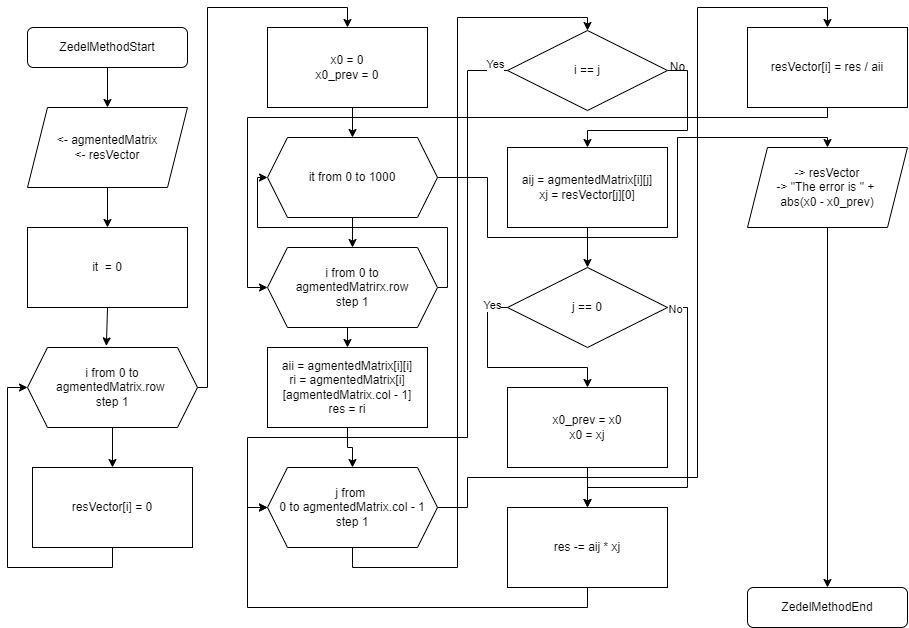
\includegraphics[width=0.9\textwidth]{AMO/img/Iteration.png }
\caption{Блок-схема алгоритму ітерацій Зеделя}
\label{fig:zedelfc}
\end{figure}

\section{Посилання на проект}

Посилання на \href{https://github.com/Folainer/university/tree/main/AMO}{git} репозіторій

\end{document}